% importa variabili globali
% definizione variabili globali
\def\GRUPPO {\textit{DazzleWorks}}

\def\PROGETTO {\textbf{Premi}}

\def\COMMITTENTE {Prof. Vardanega Tullio, \\ & Dr. Cardin Riccardo}

\def\EMAIL {dazzleworksgroup@gmail.com}

\def\LOGO {../../template/img/logo.png}

\def\INTESTAZIONE {../../template/img/intestazione.png}
\def\PIEDIPAGINA {../../template/img/piedipagina.png}

\def\G {{\small $_G$}}



% definizione variabili locali
\def\DOCUMENTO{Norme di Progetto}
\def\VERSIONE{1.0.0}

\def\DESCRIZIONE{Documento contenente l’insieme di norme stabilite dal gruppo \GRUPPO per la realizzazione del progetto didattico \PROGETTO.}

\def\REDATTORE {Suierica Bogdan \\ & Crespan Emanuele}
\def\VERIFICATORE {Agostinetto Matteo}
\def\RESPONSABILE {Burlin Valerio}

\def\USO {Interno}

\def\DISTRIBUZIONE {\GRUPPO{}\\ & \COMMITTENTE{}\\}

\def\DESCRIZIONE {Documento contenente l'insieme di norme stabilite dal gruppo \GRUPPO\ per la realizzazione di \PROGETTO.}


% abilita (true) / disabilita (false) indice, lista tabelle, lista figure
\def\INDICE	{true}
\def\TABELLE {false}
\def\FIGURE {true}


% importa struttura
\documentclass[a4paper]{article}

% ----- definizioni -----
\def\TITLE		{\mbox{\GRUPPO}}
\def\SUBTITLE	{\SIGLA, \PROGETTO}


% ----- nuovi comandi -----
% fornisce il caption per riferirsi ad una particolare sezione
\newcommand{\numref}[1]{\textsf{\textsl{``\nameref{#1}'' (\ref{#1})}}}


% ----- package -----
\usepackage[T1]{fontenc}   % codifica dei font in uscita
\usepackage[utf8x]{inputenc}   % lettere accentate da tastiera
\usepackage[italian]{babel}   % lingua principale del documento
\usepackage[a4paper, top= 3cm, bottom= 3cm, left= 3cm, right= 3cm, bindingoffset= 5mm]{geometry} % impostazione margini

\usepackage{amssymb} %

\usepackage{booktabs} % comandi aggiuntivi per le tabelle

\usepackage{calc} % espressioni aritmetiche
\usepackage{caption} % descrizione figure, ecc
\usepackage{chapterbib} % inclusione delle bibliografie

\usepackage{datatool} % manipolazione dati
\usepackage{dcolumn} % array in tabular

\usepackage{epstopdf} % conversione eps--> pdf
\usepackage{enumitem} % personalizzazione liste
\usepackage{eurosym} % simbolo euro

\usepackage{fancyhdr}   %personalizzazione dello stile
\usepackage{float} % definizione di oggetti floating (es. figure, tabelle)
\usepackage[bottom]{footmisc} % personalizzazione note

\usepackage[toc]{glossaries}	% glossario
\usepackage{graphicx, subfigure} % pacchetto grafica testo
\usepackage{grffile} % estende gestione filename graphic

\usepackage[colorlinks=true, urlcolor=blue, citecolor=black, linkcolor=black, hyperindex, breaklinks]{hyperref} % gestione dei link

\usepackage{ifthen}	% costrutto ifthenelse

% \usepackage{listings} % inserimento pezzi di codice
\usepackage{longtable} % tabelle su più pagine

\usepackage{pgf} % grafica postscript e PDF
\usepackage{pgfplots}	% composizione di grafici
\pgfplotsset{/pgf/number format/use comma, compat=newest}	% opzioni per i grafici

\usepackage{multirow} % span multiriga

\usepackage{tabularx, array} % crea paragrafi a colonne
\usepackage{titlesec} % personalizzazione titoli
\usepackage{tikz} % gestione delle formule
\usepackage{totpages} % conta numero pagine

\usepackage{soul} % gestione letterspacing
\usepackage{subfigure} % gestione delle sottofigure

\usepackage{verbatim} % inserimento testo verbatim, non interpretato

\usepackage{wallpaper} % gestione background

\usepackage{xspace} % spazi automatici per le macro


% ----- posizione etichette -----
\captionsetup{tableposition=top, figureposition=bottom, font=small}


% ----- glossario -----
\loadglsentries{../../glossario/glossario.tex}
\renewcommand*{\glssymbolsgroupname}{Simboli}


% ----- stile pagina -----
\pagestyle{fancy}

	% header
	\fancypagestyle {firststyle} {	% definizione stile "firststyle"
		\fancyhf{}
	}

	% indentazione paragrafo
	%\setlength{\parindent} {0pt}
	\setlength{\headheight} {25pt}

	% intestazione
	\lhead{}
	\rhead{\nouppercase{\leftmark}}
	\renewcommand{\headrulewidth}{0pt}  % no linea sotto intestazione

	% piè di pagina
	\lfoot{\footnotesize{{\DOCUMENTO} \\ {\VERSIONE}}}
	\cfoot{}
	\rfoot{\thepage}
	\renewcommand{\footrulewidth}{0pt}   % no linea sopra piè di pagina


% ----- inizio documento -----
% ----- prima pagina -----
\begin{document}
\thispagestyle{firststyle}

\begin{center}

%   \vspace{7cm}
	\textbf{{\fontsize{40pt}{41pt}\selectfont \PROGETTO}} \\
	\rule{8cm}{3pt}
   
   \vspace{4cm}
   \includegraphics[height= 4cm] {\LOGO}
   
	\vspace{1cm}
   {\fontsize{30pt}{31pt}\selectfont \textbf{\GRUPPO}}
	
	\vspace{5cm}
	{\fontsize{18pt}{24pt}\selectfont \textbf{\DOCUMENTO}}
	
%	\vspace{1cm}
	\begin{center}
		\begin{tabular}{r|l}
				\textbf{Versione} & \VERSIONE \\
				\textbf{Redattori} & \REDATTORE \\
				\textbf{Verificatori} & \VERIFICATORE \\
				\textbf{Responsabili} & \RESPONSABILE \\
				\textbf{Uso} & \USO \\
				\textbf{Lista di distribuzione} & \DISTRIBUZIONE
		\end{tabular}
	\end{center}

	\vspace{1cm}
	\textbf{\DESCRIZIONE}

\end{center}


\newpage

% ----- pagine successive -----
\ULCornerWallPaper{1}{\INTESTAZIONE}
\LLCornerWallPaper{1}{\PIEDIPAGINA}

%\thispagestyle{empty}

\newpage

% diario delle modifiche


% numerazione pagine indici
\pagenumbering{Roman}


\newpage
\section*{Diario delle modifiche}

\begin{table}[h]
\centering
\begin{tabular}{|p{0.3\textwidth}|c|c|c|c|}
	\toprule
		\textbf{Modifiche} & \textbf{Autore} & \textbf{Ruolo} & \textbf{Data} & \textbf{Ruolo} \\
	\midrule
	\midrule
		\textit{Approvazione documento} & Agostinetto Matteo & \textit{Responsabile di Progetto} & 2015-04-09 & v1.0.0 \\
	\midrule
		\textit{Eseguita verifica documento} & Burlin Valerio & \textit{Verificatore} & 2015-04-08 & v0.3.0 \\
	\midrule
		\textit{Modifica sezione Resoconto Attività di Verifica sulla base delle segnalazioni del verificatore} & Suierica Bogdan & \textit{Verificatore Capo} & 2015-04-08 & v0.2.1 \\
	\midrule
		\textit{Eseguita verifica documento} & Burlin Valerio & \textit{Verificatore} & 2015-04-07 & v0.2.0 \\
	\midrule
		\textit{Inserimento sezione Resoconto Attività di Verifica} & Suierica Bogdan & \textit{Verificatore Capo} & 2015-04-06 & v0.1.2 \\
	\midrule
		\textit{Modifica sezioni Visione Generale della Strategia di Verifica e Gestione Amministrativa della Revisione sulla base delle segnalazioni del verificatore} & Bogdan Suierica & \textit{Verificatore Capo} & 2015-03-20 & v0.1.1 \\
	\midrule
		\textit{Eseguita verifica documento} & Burlin Valerio & \textit{Verificatore} & 2015-03-17 & v0.1.0 \\
    \midrule
	    \textit{Completamento sezione Visione Generale della Strategia di Verifica} & Suierica Bogdan & \textit{Verificatore Capo} & 2015-03-16 & v0.0.6 \\
	\midrule
		\textit{Completamento appendice Standard di Qualità} & Crespan Emanuele & \textit{Amministratore di Progetto} & 2015-03-16 & v0.0.5 \\
	\midrule
		\textit{Completamento sezione Gestione Amministrativa della Revisione} & Crespan Emanuele & \textit{Amministratore di Progetto} & 2015-03-15 & v0.0.4 \\
	\midrule
		\textit{Completamento sezione Introduzione ed inizio stesura sezione Visione Generale della Strategia di Verifica} & Suierica Bogdan  & \textit{Verificatore Capo} & 2015-03-12 & v0.0.3 \\
	\midrule
		\textit{Inizio stesura sezione Gestione Amministrativa della Revisione} & Crespan Emanuele & \textit{Amministratore di Progetto} & 2015-03-09 & v0.0.2 \\	                         
	\midrule
		\textit{Inizio stesura sezione Introduzione e appendice Standard di Qualità} & Suierica Bogdan & \textit{Verificatore Capo} & 2015-03-09 & v0.0.1 \\
	\bottomrule
\end{tabular}	
\end{table}

\newpage

% importa indici
% definizione indice
\ifthenelse{\equal{\INDICE}{true}}
	{\tableofcontents \newpage}{}

% definizione lista tabelle
%\ifthenelse{\equal{\TABELLE}{true}} 
%	{\listoftables \newpage}{}

% definizione lista figure
\ifthenelse{\equal{\FIGURE}{true}}
	{\listoffigures \newpage}{}


% numerazione pagine
\pagenumbering{arabic}

	% formato visualizzazione
	\rfoot{\thepage ~di~\pageref{TotPages}}


% separatore
\iffalse
	AOjvdYTJD7mcIIYItfsNiYPbmTTogRSP9hrrb2XPE1laMyQ9NHrPgTCTxnW0eV1YcM3Wqh7t5qThjczeXWq3O5FJ7BBQjoWZovC5
\fi

% importa parti documento

%\section{<nomesezione>}
\section{Introduzione}
\subsection{Scopo del documento}
Il \textit{Piano di Qualifica} ha lo scopo di fissare le strategie che il gruppo intende adottare, al fine di perseguire gli obbiettivi di qualità, sia di processo che di prodotto. Per questo motivo è necessaria una costante verifica sulle attività svolte. Così facendo si permette di trovare possibili incongruenze e anomalie per poter intervenire in maniera tempestiva ed efficace.
\subsection{Scopo del prodotto}
Lo scopo del prodotto è la realizzazione di un software di presentazione di \textit{slide}, utilizzando il linguaggio HTML5, che funzioni sia su desktop che su dispositivi mobile. Si richiede di realizzare effetti grafici a supporto dello \textit{storytelling}\footnote{L'arte del raccontare storie impiegata come strategia di comunicazione.} e che sia di livello comparabile con Prezi\footnote{Software di presentazioni.}.
\subsection{Glossario}
Al fine di evitare ogni ambiguità e permettere al lettore una migliore comprensione i termini tecnici e gli acronimi sono riportati, con relativa descrizione, nel documento \textit{Glossario}. 
Ogni occorrenza di un termine appartenente al \textit{Glossario} è marcata da una \G in pedice.
\subsection{Riferimenti}
	\subsubsection{Normativi}
	\begin{itemize}
		\item \textbf{Norme di Progetto:} \textit{Norme di Progetto v1.0.0};
		\item \textbf{Capitolato d'appalto C4:} Premi: software di presentazione "better than Prezzi" \url{http://www.math.unipd.it/~tullio/IS-1/2014/Progetto/C4p.svg#1_0}.
	\end{itemize}
	\subsubsection{Informativi}
	\begin{itemize}
		\item \textbf{Piano di Progetto:} \textit{Piano di Progetto v1.0.0};
		\item \textbf{Slide Ingegneria del Software 2014/2015:} \url{http://www.math.unipd.it/~tullio/IS-1/2014/}
		\item \textbf{Indice Gulpease:} \url{http://it.wikipedia.org/wiki/Indice_Gulpease}
		\item \textbf{Standard ISO/IEC 9126:} \url{http://it.wikipedia.org/wiki/ISO/IEC_9126}
		\item \textbf{Standard ISO/IEC 15504:} \url{http://en.wikipedia.org/wiki/ISO/IEC_15504}
	\end{itemize}
\newpage
\section{Collaborazione}
	\subsection{Comunicazioni}
		\subsubsection{Comunicazioni interne}
Le comunicazioni interne verranno eseguite attraverso la mailing list: \url{dazzleworksgroup@gmail.com}. \\ 
Quando un membro del gruppo vuole inviare una email a tutti i componenti, deve inviare il messaggio dalla sua casella di posta elettronica personale verso l'indirizzo \url{dazzleworksgroup@gmail.com}, dalla quale un inoltro automatico provvederà a mandare l'email agli altri indirizzi di posta elettronica personali dei componenti del gruppo, tenendo traccia di tutte le comunicazioni.\\ 
I membri sono tenuti a prestare attenzione al numero di messaggi diffusi. È sempre importante non arrivare a una sovraesposizione del pubblico interno, in quanto si creerebbe solo senso di smarrimento e confusione. Questo non esclude che uno stesso messaggio non sia proposto su più mezzi di informazione, azione spesso necessaria, ma questo presuppone un intervento ponderato e non casuale.\\
Con lo scopo di facilitare la comunicazione tra i membri del gruppo vengono utilizzati strumenti di messaggistica istantanea e videochiamata come Skype e Google Hangouts.
È necessario redigere un \gls{verbale} nel caso in cui siano state prese decisioni o siano emersi dettagli inerenti allo sviluppo del progetto. 
		\subsubsection{Comunicazioni esterne}
Per le comunicazioni esterne è stato creato un indirizzo di posta elettronica:
\begin{center}
\url{dazzleworksgroup@gmail.com}
\end{center}
Tale indirizzo deve essere l'unico canale di comunicazione verso l'esterno. Sarà solo il \textit{Responsabile di progetto} ad utilizzare l'indirizzo di posta per intrattenere le corrispondenze con i proponenti e i Committenti. È compito del \textit{Responsabile di progetto} informare i membri del gruppo delle discussioni avvenute ed eventualmente inoltrare i messaggi alla mailing list.

	\subsection{Composizione email}
In questo paragrafo viene descritta la forma che deve avere una email sia per comunicazione interna che esterna.
		\subsubsection{Mittente}
\begin{itemize}
	\item \textbf{Interno:} indirizzo personale di chi scrive il messaggio;
	\item \textbf{Esterno:} l'unico indirizzo utilizzabile per comunicare verso l'esterno è \url{dazzleworksgroup@gmail.com} e deve essere usato esclusivamente dal \textit{Responsabile di progetto}.
\end{itemize}
	\subsubsection{Destinatario}
\begin{itemize}
	\item \textbf{Esterno:} l'indirizzo del destinatario può avere variazioni a seconda che si voglia comunicare con il Prof. Tullio Vardanega, il Prof. Riccardo Cardin o con i Proponenti del progetto;
	\item \textbf{Interno:} l'unico indirizzo utilizzabile è \url{dazzleworksgroup@gmail.com}.
\end{itemize}
Le uniche eccezioni permesse sono:
\begin{itemize}
	\item \textbf{Proposte all'\textit{Amministratore di Progetto}:} per eventuali proposte di cambiamento delle norme da parte di un membro del gruppo, quest'ultimo dovrà contattarlo al suo indirizzo di posta elettronica personale;
	\item \textbf{Comunicazione ristretta tra alcuni membri del gruppo:} in questi casi i membri del gruppo utilizzeranno i loro indirizzi personali.
\end{itemize}

		\subsubsection{Oggetto}
L'oggetto deve sintetizzare il contenuto della email. Deve essere chiaro, breve e possibilmente univoco in modo da riconoscerlo dagli altri precedenti.\\
Nel caso si debba mandare un messaggio alla mailing list è obbligatorio aggiungere "Group:" all'inizio dell'oggetto.
		\subsubsection{Corpo}
Il corpo del messaggio deve essere chiaro, diretto e avere tutte le informazioni necessarie per permettere a tutti i destinatari di capire correttamente l'argomento trattato. Per riferirsi ad alcuni componenti del gruppo o ruoli di progetto si dovrà usare la seguente sintassi: "\textbf{Cognome Nome}" o "\textbf{Nome Ruolo}". Alla fine del corpo del messaggio, il mittente dovrà sempre firmarsi con il suo nome, cognome e ruolo all'interno del gruppo.
		\subsubsection{Allegati}
Viene consentito l'uso di allegati che deve essere limitato solo al caso in cui essi siano realmente necessari. È buona norma presentare gli allegati scrivendo alcune righe di spiegazione. Prestare attenzione al formato(preferibilmente PDF) del documento che si sta inviando. 

	\subsection{Riunioni}
Il \textit{Responsabile di progetto} ha il compito di indire le riunioni, sia interne che esterne. Per ogni riunione sarà necessario specificare data, ora, luogo, e l'ordine del giorno. Le informazioni sulla riunione dovranno essere rese disponibili con almeno quattro giorni di anticipo.
		\subsubsection{Interne}
Sarà il \textit{Responsabile di Progetto} a convocare i componenti del gruppo alle riunioni generali. Tutti i membri del team dovranno partecipare fisicamente o in video chiamata Le riunioni avranno una frequenza almeno quindicinale. Ogni componente del gruppo è tenuto a leggere la posta elettronica e rispondere ad eventuali richieste di riunioni interne. \\
Il \textit{Responsabile di progetto} può anticipare o posticipare una riunione in base alla disponibilità data dai componenti del gruppo. È possibile richiedere una riunione generale da parte di un qualsiasi componente del gruppo. La richiesta verrà inoltrata al \textit{Responsabile di Progetto} che potrà decidere se accoglierla o rifiutarla.\\
Inoltre, è possibile e auspicabile che siano necessarie riunioni tra specifici membri del gruppo, ad esempio: in fase di analisi può essere utile che solo gli \textit{Analisti} si incontrino tra di loro. I componenti che non hanno preceduto la riunione saranno comunque informati sui contenuti e le decisioni prese tramite invio di una email alla mailing list o alla pubblicazione di un \gls{verbale} sul \gls{repository} nel caso siano state prese decisioni importanti.
		\subsubsection{Esterne}
Sarà il \textit{Responsabile di progetto} a fissare le riunioni esterne con i Proponenti e/o i Committenti utilizzando la casella di posta creata appositamente. Prima di contattare le parti esterne, il \textit{Responsabile di progetto} dovrà verificare la presenza dei membri interni al gruppo. \\
In caso di risposta positiva si provvederà a contattare i Proponenti e/o i Committenti per fissare la data dell'incontro.
È compito del \textit{Responsabile di progetto} a redigere il \gls{verbale} dell'incontro avvenuto.

	\subsection{Verbale}
Per verbali si intende quanto si è discusso nel corso di una riunione e le decisioni che eventualmente sono state assunte. \\
Nella stesura di un \gls{verbale} occorre essere sintetici, essenziali ed esaustivi, cercando di rappresentare gli interventi, le osservazioni o le decisioni assunte in maniera oggettiva, senza interpretazioni personali, ambigue o fuorvianti. Il tempo dei verbi che deve essere utilizzato è il presente.\\
I verbali dovranno obbligatoriamente includere le seguenti informazioni:
\begin{itemize}
	\item Dove e quando si svolge la riunione, i partecipanti, gli assenti, il nome di chi presiede e quello del segretario verbalizzante;
	\item Tipo di incontro(interno o esterno);
	\item Le questioni e/o i problemi ancora irrisolti;
	\item I (nuovi) argomenti posti in discussione all'ordine del giorno;
	\item Gli interventi più significativi rappresentati in ordine temporale; 
	\item I suggerimenti, le proposte, le conclusioni e le decisioni assunte; 
	\item I compiti assegnati ad ognuno con indicazione delle rispettive scadenze; 
	\item Gli argomenti da trattare nella prossima riunione. 
\end{itemize}

	\subsection{Repository}\label{repository}
In questa sezione sono definiti gli strumenti utilizzati per la condivisione dei file. \\
Per la gestione della documentazione e della codifica è stato creato un \gls{repository}. Il \gls{repository} è privato e quindi accessibile solo dai membri del gruppo \GRUPPO.\\
Dopo l'ultima revisione il progetto verrà reso open-source.
Per il \gls{repository} abbiamo scelto di usare il servizo \gls{GitHub}, il quale utilizza il sistema di \gls{versionamento} \gls{Git}.
		\subsubsection{Utilizzo del servizio}
È necessario eseguire le operazioni di sincronizzazione all'inizio e alla fine di ogni sessione di lavoro. \\
In particolare ad ogni sessione di lavoro andranno eseguite le seguenti operazioni:
\begin{itemize}
	\item \textbf{Pull} - scaricare da la versione più aggiornata del progetto per poterci poi lavorare offline;
	\item \textbf{Add} - aggiungere i file ad uno specifico elenco generando una proposta di modifica;
	\item \textbf{Commit} - validare le proposte fatte in precedenza;
	\item \textbf{Push} - serve a pubblicare i risultati online, sulla piattaforma di sviluppo;
	\item \textbf{Merge} - permette di fondere un \gls{branch} con il \gls{repository} padre, così da implementare le modifiche apportate ai file e alle cartelle originarie.
\end{itemize}
È vietato utilizzare "git add *" per evitare di includere file nascosti essendo consapevoli dell'esatto contenuto. Ogni commit deve essere corredato di un messaggio che descriva in modo \gls{conciso} il lavoro svolto.

		\subsubsection{Struttura}
Tutta la documentazione si può trovare in un \gls{repository} disponibile al seguente indirizzo: \url{https://github.com/FabioRos/Premi}. \\
Esso avrà questa struttura:
\begin{itemize}
	\item \textbf{Interni:}
		\begin{itemize}
				\item \textbf{Studio di fattibilità};
				\item \textbf{Norme di Progetto}.
		\end{itemize}
	\item \textbf{Esterni:}
		\begin{itemize}
				\item \textbf{Analisi dei Requisiti};
				\item \textbf{Piano di progetto};
				\item \textbf{Piano di qualifica};
				\item \textbf{Glossario};
				\item \textbf{Lettera di presentazione};
				\item \textbf{Verbali}.
		\end{itemize}
\end{itemize}



\newpage
\section{Ruoli di Progetto}
Lo sviluppo prevede la collaborazione di individui a cui verranno assegnati ruoli diversi. Tali ruoli rappresentano figure aziendali specializzate, indispensabili per il buon esito del progetto.\\
Di seguito i diversi ruoli di progetto con le relative responsabilità e modalità operative.
\subsection{Responsabile di Progetto}
Il \textit{Responsabile di Progetto} rappresenta il progetto, in quanto accentra su di sé la responsabilità di scelta e approvazione, ed il gruppo, poiché presenta al committente i risultati del lavoro svolto.
Detiene il potere decisionale, quindi la responsabilità in merito a:
\begin{itemize}
	\item Pianificazione, coordinamento e controllo delle attività;
	\item Gestione e controllo delle risorse;
	\item Analisi e gestione dei rischi;
	\item Approvazione dei documenti;
	\item Approvazione dell'offerta economica.
\end{itemize}
Di conseguenza, ha il compito:
\begin{itemize}
	\item Assicurarsi che le attività di verifica e validazione vengano svolte sistematicamente seguendo le \textit{Norme di Progetto v2.0.0};
	\item Garantire che vengano rispettati i ruoli e le competenze assegnate nel \textit{Piano di Progetto};
	\item Garantire che non vi siano conflitti tra \textit{Verificatori} e \textit{Redattori};
	\item Gestire la creazione e l'assegnazione dei \gls{ticket} ad ogni membro del gruppo.
\end{itemize}
\subsection{Ammministratore}
L'\textit{Amministratore di Progetto} è il responsabile dell'efficienza e del rendimento nell'ambiente di lavoro. Le mansioni che gli competono sono le seguenti:
\begin{itemize}
	\item Agevolare le attività richieste dalle \textit{Norme di Progetto v2.0.0};
	\item Ricercare e rendere operativi tutti gli strumenti necessari all'automatizzazione del maggior numero di compiti;
	\item Fornire procedure e strumenti per il controllo e la segnalazione del controllo qualità;
	\item Gestire l'archiviazione e il \gls{versionamento} della documentazione;
	\item Controllare le versioni dei prodotti e gestire le loro configurazioni.
\end{itemize}
Redige le \textit{Norme di Progetto}, dove spiega e norma l'utilizzo degli strumenti, e redige la sezione del \textit{Piano di Qualifica} dove vengono descritti strumenti e metodi di verifica.
\subsection{Analista}
L'\textit{Analista} è il responsabile delle attività di analisi. Le mansioni che gli competono sono:
\begin{itemize}
	\item Comprendere appieno la natura e la complessità del problema;
	\item Produrre una \textit{specifica di progetto} motivata in ogni suo punto e comprensibile a tutti gli interessati.
\end{itemize}
Redige lo \textit{Studio di Fattibilità}, l'\textit{Analisi dei Requisiti} e partecipa alla redazione del \textit{Piano di Qualifica} in quanto conosce l'ambito di progetto.

\subsection{Progettista}
Il \textit{Progettista} è il responsabile delle attività di progettazione. La mansioni che gli competono sono:
\begin{itemize}
	\item Produrre una soluzione comprensibile, attuabile e motivata;
	\item Effettuare scelte su aspetti progettuali che applichino al prodotto soluzioni note ed ottimizzate;
	\item Effettuare scelte su aspetti progettuali e tecnologici che rendano il prodotto facilmente manutenibile.
\end{itemize}
Redige la \textit{Specifica Tecnica}, la \textit{Definizione di Prodotto} e le sezioni relative alle metriche di verifica della programmazione del \textit{Piano di Qualifica}.

\subsection{Verificatore}
Il \textit{Verificatore} è il responsabile delle attività di verifica. Le mansioni che gli competono sono:
\begin{itemize}
	\item Garantire che l'attuazione delle attività sia conforme alle norme stabilite;
	\item Verificare che non siano stati introdotti errori lungo il percorso;
	\item Controllare la conformità di ogni stadio del ciclo di vita del prodotto.
\end{itemize}
Redige la sezione del \textit{Piano di Qualifica} che illustra l'esito e la completezza delle verifiche
e delle prove effettuate.

\subsection{Programmatore}
Il \textit{Programmatore} è responsabile delle attività di codifica e delle componenti di ausilio necessarie per l'esecuzione delle prove di verifica e validazione. Le mansioni che gli competono sono:
\begin{itemize}
	\item Implementare in maniera rigorosa le soluzioni descritte dal \textit{Progettista};
	\item Scrivere codice che sia documentato, versionato, manutenibile e che rispetti le metriche stabilite per la scrittura del codice;
	\item Implementare i test sul codice prodotto, necessari per le prove di verifica e validazione.
\end{itemize}
Redige il \textit{Manuale Utente}.

\subsection{Rotazione dei ruoli}
Ogni membro del gruppo dovrà ricoprire tutti i ruoli definiti nel \textit{Piano di Progetto v2.0.0}. Il \textit{Responsabile di Progetto} avrà il compito di pianificare l'impiego delle risorse in modo equo e in modo che ogni risorsa ricopra tutti i ruoli. 
Si deve controllare attentamente che non vi siano conflitti di interesse specialmente nelle attività di approvazione e verifica. Per garantire che la rotazione dei ruoli non provochi conflitti è necessario che le attività vengano pianificate con attenzione e che i membri interessati rispettino ruoli e compiti loro assegnati. Spetterà al \textit{Verificatore} controllare che tutte le condizioni sopra indicate vengano rispettate. Se il \textit{Verificatore} troverà delle incongruenze con quanto menzionato sopra avrà il compito di avvisare il \textit{Responsabile di Progetto} che dovrà risolvere la questione.\\
Ogni componente del gruppo potrà consultare, in qualsiasi momento, i diagrammi di \gls{Gantt} che descrivono la gestione delle risorse e dei ruoli, in maniera tale che ognuno potrà sempre essere consapevole del ruolo ricoperto dagli altri componenti.


\newpage
\section{Documenti}
\section{Documenti}
In questo capitolo si descrivono i vari standard adottati da \GRUPPO nella stesura, verifica e approvazione della documentazione da produrre.
\subsection{Template}
Per semplificare la redazione dei documenti è stato creato un template \LaTeX contenente tutte le impostazioni per l'aspetto grafico. \\
Ogni documento dovrà essere realizzato con il template \LaTeX presente nel \gls{repository}. Inoltre è stata scritta una piccola una piccola guida su come usare al meglio il template.
\subsection{Versionamento}
Per ogni documento è obbligatorio specificare la versione. Un numero di versione deve essere nella seguente forma:
\begin{center}
	\emph{X.Y.Z}
\end{center}
dove X, Y, Z sono interi non negativi e non devono contenere zeri iniziali. X è la versione \textit{Major}, Y è la versione \textit{Minor}, e Z e la versione \textit{Patch}.
\begin{itemize}
	\item X: la versione Major (X.y.z | X > 0) identifica la versione di rilascio. Deve essere incrementata se è stata introdotta qualsiasi modifica non retrocompatibile. Le versioni Patch e Minor devono essere reimpostate a 0 quando la versione Major è incrementata. 
	\item Y: la versione Minor (x.Y.z | x > 0) deve essere incrementata se è stata introdotta una nuova funzionalità. La versione Patch deve essere reimpostata a 0 quando la versione Minor è incrementata.
	\item Z: la versione Patch (x.y.Z | x > 0) deve essere incrementata solo se sono state introdotte correzioni retrocompatibili di bug. Una correzione di un bug è definita come una modifica interna che corregge un comportamento errato.
\end{itemize}
Una volta che un pacchetto versionato è stato rilasciato, i contenuti di quella versione \textbf{non devono} essere modificati. Qualsiasi modifica \textbf{deve} essere rilasciata come una nuova versione.

\subsection{Struttura dei documenti}
\subsubsection{Prima pagina}
Ogni documento deve avere in prima pagina le seguenti informazioni:
\begin{itemize}
	\item Nome del progetto;
	\item Logo del gruppo;
	\item Nome del gruppo;
	\item Nome del documento;
	\item La versione del documento;
	\item Cognome e nome dei redattori del documento;
	\item Cognome e nome dei verificatori del documento;
	\item Cognome e nome di chi ha approvato il documento;
	\item Tipo d'uso del documento;
	\item Lista di distribuzione del documento;
	\item Breve descrizione del documento.
\end{itemize}
\subsubsection{Diario delle modifiche}
Nella seconda pagina di ogni documento deve essere presente il diario delle modifiche.\\
Ogni riga del diario delle modifiche contiene:
\begin{itemize}
	\item Una breve descrizione sulle modifiche effettuate;
	\item Cognome e nome di chi ha effettuato la modifica;
	\item Data della modifica;
	\item Versione del documento dopo la modifica.
\end{itemize}

\subsubsection{Indice}
In ogni documento deve essere presente un indice delle sezioni.\\
Nel caso in cui il documento contenga immagini e/o tabelle devono essere presenti anche i relativi indici.

\subsubsection{Formattazione delle pagine}
L'intestazione di ogni pagina contiene:
\begin{itemize}
	\item Logo del gruppo;
	\item La sezione corrente all'interno del documento.
\end{itemize}
A piè di ogni pagina è presente:
\begin{itemize}
	\item Nome e versione del documento;
	\item Pagina corrente nel formato N di T, dove N è il numero della pagina corrente e T è il numero di pagine totali del documento.
\end{itemize}

\subsection{Classificazione documenti}
\subsubsection{Documenti informali}
Si definiscono documenti informali tutti i documenti in fase di sviluppo e devono ancora essere approvati dal \textit{Responsabile di Progetto}. I documenti sono da considerarsi esclusivamente per uso interno e non potranno essere divulgati prima di essere stati verificati ed approvati. 
\subsubsection{Documenti formali}
Si definiscono documenti formali tutti i documenti che sono stati approvati dal \textit{Responsabile di Progetto} e quindi sono pronti ad essere diffusi a terze parti.\\
I documenti pronti per il rilascio dovranno essere rinominati osservando le seguenti regole:
\begin{itemize}
	\item La prima lettera di ogni parola, che non sia una preposizione, deve essere maiuscola;
	\item Gli spazi devono essere sostituiti con il carattere "\_"(underscore);
	\item Tutte le parole devono essere prive di accenti;
	\item La versione del documento verrà aggiunta dopo il nome, e sarà preceduta dal carattere "-"(trattino) e da una "v".
\end{itemize}

\subsection{Norme tipografiche}
Questa sezione racchiude tutte le informazioni riguardanti l'ortografia, la tipografia e l'assunzione di uno stile uniforme in tutti i documenti allo scopo di evitare incoerenze tra le diverse parti del documento.

\subsubsection{Punteggiatura}
\begin{itemize}
	\item Punteggiatura: qualsiasi carattere di punteggiatura non può seguire un carattere di spazio;
	\item Lettere maiuscole: l'uso delle maiuscole è obbligatorio in una serie di casi:
	\begin{itemize}
		\item All'inizio di testo o di una sua parte (capitolo, paragrafo, ecc.);
		\item Dopo il punto, il punto esclamativo, il punto interrogativo;
		\item All'inizio di ogni elemento di un elenco puntato;
		\item Per i ruoli, di progetto, i nomi dei documenti, le fasi di progetto, revisioni di progetto oltre che dove previsto dalla lingua italiana.
	\end{itemize}
	\item Parentesi: il testo racchiuso dentro le parentesi non deve mai iniziare per un carattere di spazio e non deve mai terminare con un carattere di spazio o punteggiatura.
\end{itemize}	

\subsubsection{Stile del testo}
\begin{itemize}
	\item Maiuscolo: l'uso delle maiuscolo è limitato alla trascrizione dei acronimi;
	\item Grassetto: l'uso del grassetto deve essere utilizzato nei seguenti casi: 
	\begin{itemize}
		\item Elenchi puntati: per evidenziare l'oggetto trattato;
		\item Altri casi: è possibile utilizzare il grassetto per evidenziare parole chiave.
	\end{itemize}
	\item Corsivo: l'uso del corsivo deve essere utilizzato nei seguenti casi:
	\begin{itemize}
		\item Citazioni: ogni citazione deve essere scritta in corsivo; 
		\item Documenti: ogni riferimento ad un documento deve essere scritto in corsivo (esempio: \textit{Glossario});
		\item Ruoli: ogni riferimento a figure particolari deve essere scritto in corsivo (esempio: \textit{Verificatore});
		\item Altri casi: è possibile utilizzare il corsivo per evidenziare parole particolarmente significative.
	\end{itemize}
	\item \LaTeX: ogni riferimento a \LaTeX va scritto tramite il comando \verb|\LaTex|.
\end{itemize}

\subsubsection{Composizione del testo}
\begin{itemize}
	\item Elenchi puntati: per redigere un elenco si qualificano gli elementi e si introducono mediante
	i due punti. Dopo i due punti devi andare a capo. Ogni elemento dell'elenco termina con un punto e virgola, eccetto l'ultimo che termina con un punto semplice;
	\item Pedice "G": il pedice "G" viene utilizzato in presenza di termini presenti nel \textit{Glossario};
	\item Note a piè di pagina: ogni nota deve iniziare con la lettera della prima parole maiuscola e non deve essere preceduta dal alcun carattere di spazio. Ogni nota deve terminare con un punto.
\end{itemize}

\subsubsection{Formati ricorrenti}
\begin{itemize}
	\item Nomi propri: l'utilizzo dei nomi propri deve seguire la seguente forma "Cognome Nome";
	\item Percorsi: per gli indirizzi email e gli indirizzi web deve essere usato esclusivamente il comando \LaTeX  \verb|\url|;
	\item Date:  ogni data deve seguire lo standard internazionale per date ed orari ISO 8601:
	\begin{center}
		AAAA.MM.GG
	\end{center}
	dove:
	\begin{itemize}
		\item AAAA: rappresenta il formato dell'anno scritto con quattro cifre;
		\item MM: rappresenta il formato del mese scritto con due cifre;
		\item GG: rappresenta il formato del giorno scritto con due cifre.
	\end{itemize}
	\item Riferimenti ai documenti: ci si riferirà ai vari documenti scrivendo in corsivo il nome del documento e mettendo una lettera maiuscolo per ogni parola che non sia un articolo. Nel caso in cui ci si deve riferire ad una versione specifica del documento, essa andrà indicata alla fine  del nome del documento (esempio: \textit{Norme di Progetto v1.0.0});
	\item Nome del gruppo: ci si riferirà al gruppo solo come "\textit{DazzleWorks}" con il nome del gruppo in corsivo. Per una scrittura corretta del nome è stato creato il comando \LaTeX apposito \verb|\GRUPPO|;
	\item Nome del progetto: ci si riferirà al nome del progetto solo come "\textbf{PREMI}". Per una scrittura corretta del nome è stato creato il comando \LaTeX \verb|\PROGETTO|.
\end{itemize}

\subsubsection{Sigle}
Le sigle potranno essere utilizzate esclusivamente all'interno delle tabelle e diagrammi. Sono presenti le seguente sigle: 
\begin{itemize}
	\item Documenti:
	\begin{itemize}
		\item NdP = \textit{Norme di Progetto};
		\item AdR = \textit{Analisi dei Requisiti};
		\item PdP = \textit{Piano di Progetto};
		\item PdQ = \textit{Piano di Qualifica};
		\item SdF = \textit{Studio di Fattibilità}.
	\end{itemize}
	\item Revisioni:
	\begin{itemize}
		\item RR = \textit{Revisione dei Requisiti};
		\item RP = \textit{Revisione di Progettazione};
		\item RQ = \textit{Revisione di Qualifica};
		\item RA = \textit{Revisione di Accettazione}.
	\end{itemize}
\end{itemize}

\subsection{Componenti grafiche}
\subsubsection{Immagini}
Tutte le immagini dovranno avere il formato \gls{PDF}. In modo da garantire una maggiore qualità dell'immagine in caso di ridimensionamento è consigliato usare il formato \gls{PDF} vettoriale. La conversione di un immagine in formato \gls{PDF} è possibile attraverso il software GIMP\footnote{GNU Image Manipulation Program è un programma per la creazione e modifica di immagini digitali.}, il quale è stato già usato da tutti  i componenti del gruppo. \\ Le immagini devono essere accompagnate da una didascalia che inizia con la parola "Figura" con la prima lettera maiuscola, seguita dal numero della figura, dal carattere "due punti" e da una breve descrizione della figura.
\subsubsection{Tabelle}
Ogni tabella deve essere accompagnata da una didascalia che inizia con la parola "Tabella" con la prima lettera maiuscola, seguita dal numero della tabella, dal carattere "due punti" e da una breve descrizione non banale della tabella.

\subsection{Procedure di avanzamento di un documento}
Quando il redattore ritiene di aver finito la stesura di un documento si devono seguire questi passi esattamente in quest'ordine:
\begin{enumerate}
	\item Il redattore ha il compito di contattare il \textit{Responsabile di Progetto} per informarlo della terminazione della stesura del documento;
	\item Il \textit{Responsabile di Progetto} provvederà a contattare ed assegnare la verifica del documento ad un verificatore disponibile, che non sia in conflitto di interessi;
	\item Il \textit{Verificatore} provvederà alla  verifica del documento;
	\item Nel caso in cui vengano trovati errori nel documento, il \textit{Verificatore} provvederà alla creazione di un ticket di correzione e lo assegnerà al redattore, il quale correggerà gli errori trovati e infine si tornerà di nuovo al passo uno;
	\item Se non sono stati trovati errori, il documento verrà approvato dal \textit{Responsabile di Progetto}. 
\end{enumerate}

\newpage
\section{Ambiente Lavoro}
In questa sezione verrà illustrato l'ambiente di lavoro che sarà utilizzato durante lo sviluppo del progetto \PROGETTO.\\

\subsection{Sistema operativo}

Il sistema operativo utilizzato è lasciato a discrezione di ogni membro del gruppo. Questa scelta è dovuta principalmente al fatto che il progetto dovrà supportare più piattaforme.
I membri del gruppo utilizzeranno i seguenti sistemi operativi:

\begin{itemize}
	\item \gls{Windows} 7 64 bit;
	\item \gls{Windows} 8.1;
	\item \gls{Ubuntu} 14.10;
	\item Mac OS 10.10.2.
\end{itemize}

\subsection{Coordinamento}

Il coordinamento del gruppo avviene tramite:
\begin{itemize}
	\item \gls{Repository} \gls{Git};
	\item \gls{Google Drive};
	\item \gls{Google Calendar};
\end{itemize}

\subsubsection{Repository Git}

Nonostante siano disponibili molti \gls{repository} (\gls{Git}, \gls{Mercurial}, \gls{SVN}) è stato scelto di utilizzare \gls{Git} in quanto il servizio soddisfa pienamente le necessità di \gls{hosting} e \gls{versionamento} necessarie per lo sviluppo di questo progetto, inoltre diversi membri del gruppo avevano già usato tale servizio. Esso permette di lavorare senza una connessione attiva a internet e da la possibilità di ignorare alcune estensioni specificate in un file chiamato .gitignore\footnote{File globale di \gls{Git} che contiene una lista di regole per ignorare i file.}.\\ Per i membri del gruppo che desiderano utilizzare un client, si consigliano i seguenti:
\begin{itemize}
	\item \textbf{SourceTree};
	\item \textbf{\gls{GitHub}};
\end{itemize}
Per maggiori dettagli si rimanda alla sezione \ref{repository}.

\subsubsection{\gls{Google Drive}}

Abbiamo scelto di utilizzare questo \gls{servizio cloud} per condividere tutti i documenti che non necessitano di \gls{versionamento} e vengono utilizzati frequentemente da parte dei membri del gruppo. 
È un servizio molto semplice e accessibile direttamente da \gls{browser} che permette di lavorare su documenti creati con \gls{Google Docs}.

\subsubsection{Google Calendar}
\gls{Google Calendar} viene utilizzato per la gestione delle risorse umane e per tenere traccia degli eventi importanti; infatti è stato creato un calendario condiviso con tutti i membri del gruppo in modo da conoscere le date in cui una persona è assente o non reperibile e le date rilevanti per il gruppo.\\
Inoltre è possibile modificare la gestione delle notifiche per un evento o più eventi in modo che venga inviata automaticamente una email a tutti i membri del gruppo. In questo caso il preavviso deve essere di almeno un giorno.

\subsection{Ambiente documentale}

\subsubsection{Stesura documenti}

Per la stesura dei documenti verrà utilizzato il \gls{linguaggio di markup} \LaTeX.
Come editor è consigliato TeXstudio\footnote{\url{http://texstudio.sourceforge.net}}, il quale è disponibile per tutti i principali sistemi operativi.

\subsubsection{Script}

Per facilitare la stesura dei documenti sono stati creati alcuni script:

\begin{itemize}
	\item Generazione di tutti i documenti PDF: con il comando make all verranno generati tutti i PDF dei documenti contenuti nella directory corrente;
	%\item Controllo ortografico: con il comando make aspell verrà invocato il programma aspell su tutti i documenti della directory corrente;
	%\item Eliminazione file errati o vecchi: con il comando make clean verranno eliminatati i file generati da compilazioni vecchio o file non necessari della directory corrente;
	\item Evidenziare glossario: con il comando \textit{java glossary} verrà eseguito uno script che selezionerà nei documenti, della directory corrente, le parole contenute nella versione più recente del glossario e le evidenzierà con il simbolo "\G".

\end{itemize}

\subsubsection{Pianificazione delle attività}
Per pianificare le attività e la gestione del progetto e delle risorse umane si è scelto di usare GanttProject\footnote{\url{http://www.ganttproject.biz}}.

\subsection{Ambiente di sviluppo}
Secondo il decreto legislativo n.81, ogni centoventi minuti passati in maniera continuativa davanti al computer il ogni membro deve fare almeno quindici minuti interruzione.\footnote{\url{http://www.pmi.it/impresa/normativa/news/51788/dipendenti-al-pc-obblighi-di-legge-per-i-datori-di-lavoro.html}}

\subsection{Diagrammi UML}

Per la realizzazione dei diagrammi \gls{UML} è stato scelto \gls{Astah} Professional Edition\footnote{\url{http://astah.net/download}}.
E' possibile ricevere gratuitamente la licenza della versione professional inviando una richiesta al sito \url{http://astah.net/student-license-request}.

\subsection{Verifica}

\subsubsection{Verifica dei documenti}

La verifica dei documenti verrà eseguita ogni volta che è stata effettuata una modifica ad un documento e debba essere approvato.
Per una corretta verifica di un documento vanno seguite le seguenti pratiche:

\begin{itemize}
	\item \textbf{Controllo tipografico: }tramite l'utilizzo di TeXstudio verranno individuati errori tipografici presenti nel documento;
	\item \textbf{Controllo lessicale: }il \textit{Verificatore} dovrà controllore che il documento non presenti errori lessicali attraverso un'attenta analisi del testo utilizzando la tecnica \gls{inspection} o \gls{walkthrough};
	\item \textbf{Controllo glossario: }il \textit{Verificatore} dovrà controllore che ogni parola, nel testo, presente nel glossario sia correttamente evidenziata;
	\item \textbf{Controllo contenuto: }il \textit{Verificatore} dovrà controllare che il documento contenga tutto il necessario e che sia impaginato adeguatamente;
	\item \textbf{Rispetto delle norme del progetto: }il \textit{Verificatore} dovrà controllare che il documento segua le norme di progetto stabilite;
	\item \textbf{Lista di controllo: }si dovrà stilare una lista di errori più frequenti, per semplificare le successive verifiche dei documenti;
	\item \textbf{Rispetto \gls{indice Gulpease}: }il \textit{Verificatore} dovrà calcolare e controllare, per ogni documento, che gli \gls{indici di Gulpease} risiedano nel range di valori specificato nel \textit{Piano di Qualifica}, altrimenti si dovrà effettuare una ricerca \gls{walkthrough} alla ricerca delle frasi troppo lunghe e complesse;
	\item \textbf{Segnalazione errori: }una volta completata la verifica di un documento, se sono stati riscontrati errori, il \textit{Verificatore} dovrà aprire dei \gls{ticket} per segnalarli.
\end{itemize}

\subsection{Verifica dei diagrammi}

I diagrammi devono essere verificati manualmente dal \textit{Verificatore} e deve controllare che aderiscano correttamente allo standard \gls{UML} 2.0.
In particolare deve controllare che i diagrammi di flusso siano rappresentati in maniera corretta e che i \gls{casi d'uso} utilizzino correttamente le inclusioni e le estensioni.



\newpage
\section{Protocolli e Gestione di Progetto}
Si è deciso di utilizzare il servizio di gestione dei task e creazione di milestone offerto da GitHub. Questo permette di accentrare le informazioni in un solo ambiente.\\

\subsection{Creazione e gestione dei ticket}

I ticket vengono creati e gestiti quasi tutti dal responsabile di progetto.
Qualora il \textit{verificatore} trovasse imprecisioni o errori durante la verifica, avrà la possibilità di creare dei ticket per segnalare suddetti errori.
Ogni ticket può essere assegnato ad uno o più membri del gruppo a seconda della complessità del lavoro e della disponibilità dei membri del gruppo.
Per creare un nuovo ticket bisogna:

\begin{itemize}
	\item Posizionarsi alla voce Issue;
	\item Premere "New issue";
	\item Compilare i campi richiesti:
		\begin{itemize}
			\item \textbf{Titolo e commenti:} titolo descrittivo con una descrizione del nuovo ticket;
			\item \textbf{Labels:} dovranno avere due caratteristiche fondamentali e cioè la tipologia di ticket assegnato(modifica, verifica, richiesta approvazione) e la priorità assegnata(alta, media, bassa);
			\item \textbf{Milestone:} la milestone a cui è associato il ticket;
			\item \textbf{Assignee:} a chi viene assegnato il ticket.
		\end{itemize}
\end{itemize}
\begin{figure}[h]
\centering
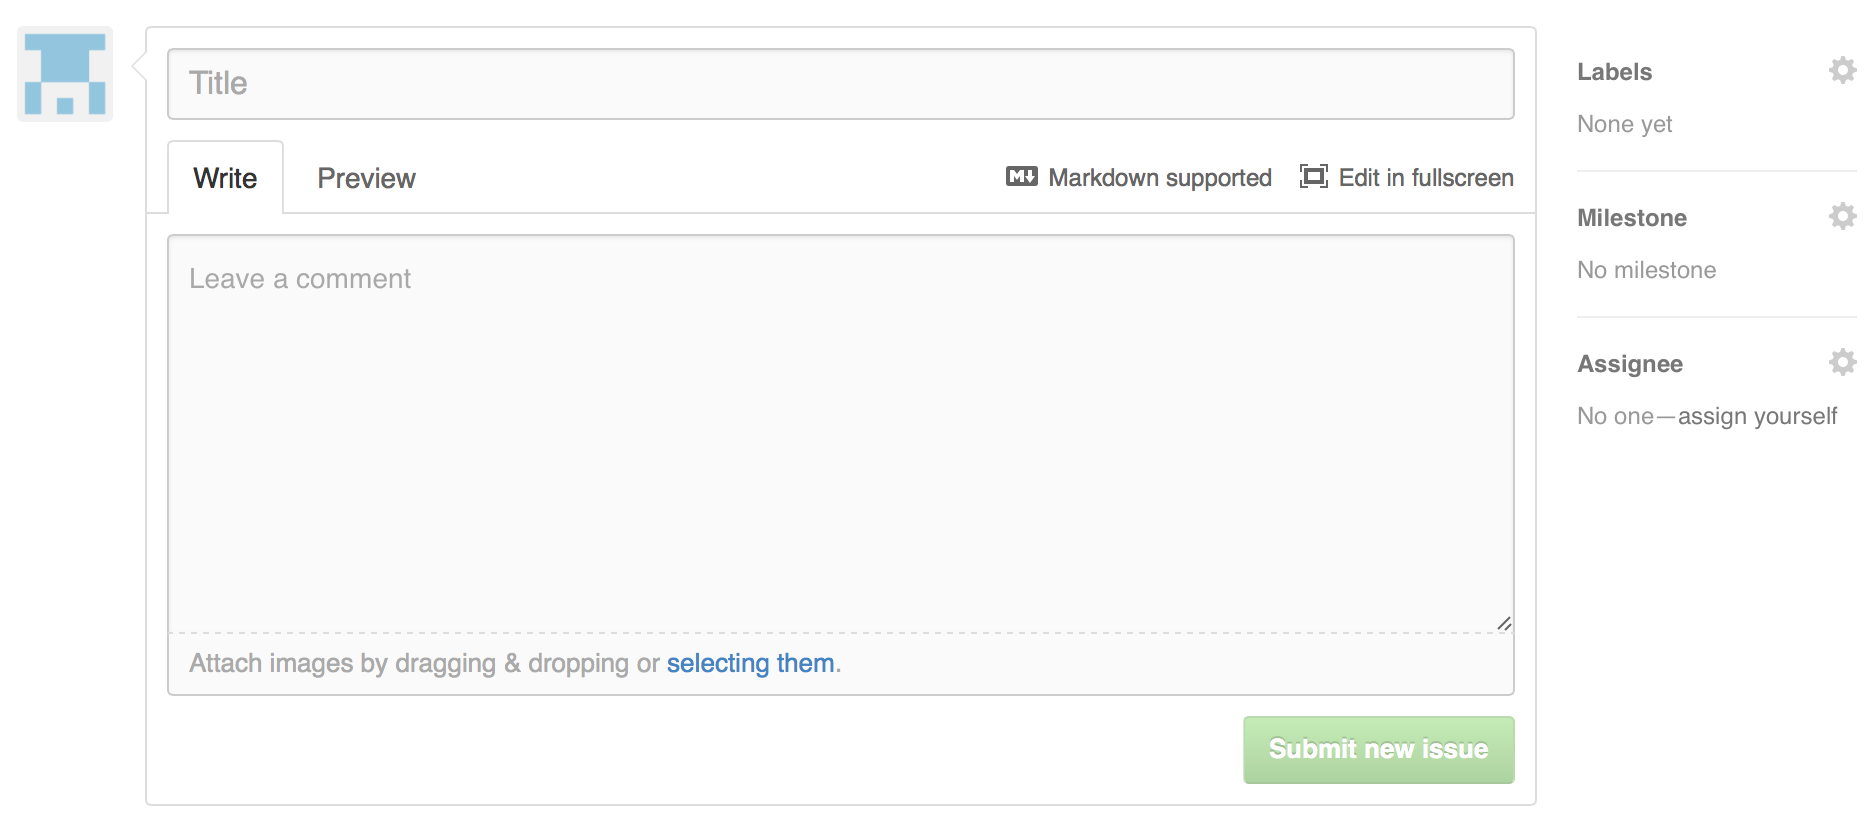
\includegraphics[width=0.7\linewidth]{img/ticket}
\caption[Creazione ticket]{Creazione ticket}
\label{fig:ticket}
\end{figure}


\subsection{Creazione delle milestone}

Il responsabile di progetto ha il compito della creazione di una milestone in occasione di ogni revisione al quale il gruppo \GRUPPO\ ha intenzione di partecipare, più altre milestone qualora il responsabile di progetto lo ritenga necessario.

Per creare una nuova milestone bisogna:

\begin{itemize}
	\item Posizionarsi alla voce Milestone;
	\item Premere "New milestone";
	\item Compilare i campi richiesti:
		\begin{itemize}
			\item \textbf{Titolo;}
			\item \textbf{Descrizione;}
			\item \textbf{Data.}
		\end{itemize}
\end{itemize}
\begin{figure}[h]
\centering
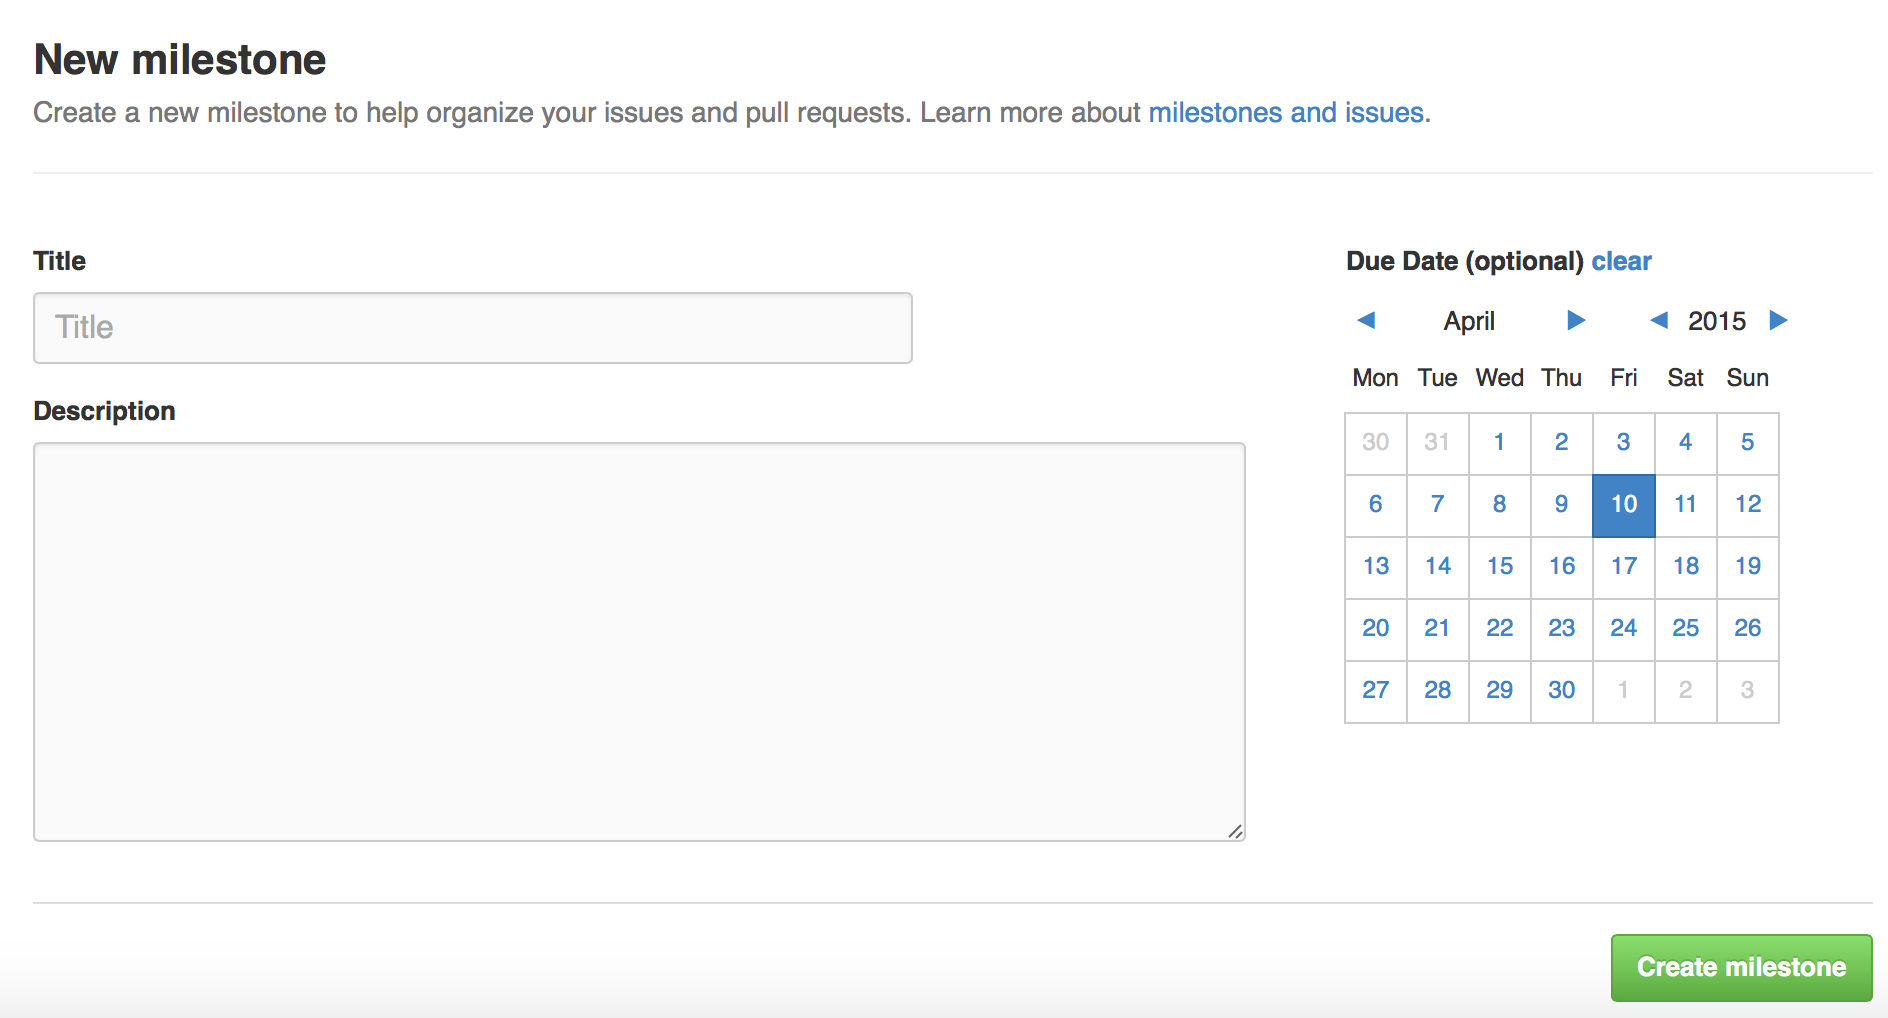
\includegraphics[width=0.7\linewidth]{img/milestone}
\caption[Creazione milestone]{Creazione milestone}
\label{fig:milestone}
\end{figure}


\subsection{Esecuzione dei compiti}

Ogni membro del gruppo è tenuto a visionare regolarmente la presenza di ticket a lui assegnati e segnalarne la presa in consegna.
Una volta che un membro porta a termine un ticket deve modificarne lo stato per segnalare il termine del lavoro.
Se un ticket non ha avuto i risultati attesi il \textit{Responsabile di Progetto} può riaprirlo ed eventualmente assegnare altri membri al lavoro.

\subsection{Chiusura della milestone}

Una volta raggiunta la scadenza, il \textit{Responsabile di Progetto}, deve chiudere la milestone ed eventualmente aprirne un'altra per poi ricominciare tutto il protocollo da capo.

\newpage
\section{Analisi Requisiti}
E' compito degli \textit{Analisti} stilare il documento \textit{Analisi dei requisiti}.
In questo documento dovranno essere presenti tutti i requisiti ed i \gls{casi d'uso} emersi dall'analisi del capitolato e dalle riunioni con il Proponente.\\

\subsubsection{Requisiti}

I requisiti dovranno essere classificati per tipo e priorità, utilizzando la seguente notazione:

\begin{center}
\begin{math}
R \left [ importanza \right ] \left [ tipo\right ]\left [codice\right ]
\end{math}
\end{center}
\begin{itemize}
  \item Importanza può assumere i seguenti valori:
\begin{itemize}
	\item \textbf{OBB:} Requisito obbligatorio;
	\item \textbf{DES:} Requisito desiderabile;
	\item \textbf{OPZ:} Requisito opzionale.
\end{itemize}
  \item Tipo può assumere i seguenti valori:
\begin{itemize}
	\item \textbf{F:} Requisito funzionale;
	\item \textbf{Q:} Requisito di qualità;
	\item \textbf{P:} Requisito di prestazione;
	\item \textbf{V:} Requisito di vincolo.
\end{itemize}
  \item Codice rappresenta il codice univoco di ogni requisito in forma gerarchica.
\end{itemize}
Ogni requisito dovrà essere inserito (nel documento \textit{Analisi dei Requisiti}) in una tabella contenente il codice identificativo, una breve descrizione e la fonte.

\subsubsection{Casi d'uso}

Dopo la stesura dei requisiti è sempre compito degli analisti analizzare i \gls{casi d'uso} (abbreviati con UC, use case).
Per ogni caso d'uso sono richieste le seguenti informazioni:
\begin{itemize}
	\item \textbf{Attori:} gli attori coinvolti nel caso d'uso (principali e secondari);
	\item \textbf{Scodo e descrizione:} una breve descrizione chiara e dettagliata del caso d'uso;
	%\item Codice identificativo: nel formato UCxx, dove xx indica un numero identificativo del caso d'uso;
	%\item Titolo: titolo sintetico del caso d'uso;
	\item \textbf{Precondizione:} la precondizione del requisito;
	\item \textbf{Flusso degli eventi:} specificare per ogni evento: descrizione, attori coinvolti e se lo scenario è descritto in dettaglio da un altro caso d'uso;
	%\item Diagramma: dovrà essere usato \gls{UML} 2.4 per la creazione dei diagrammi dei \gls{casi d'uso};
	\item \textbf{Postcondizione:} la postcondizione del requisito.
\end{itemize}
\newpage
\subsubsection{Tracciamento}
Per il tracciamento dei requisiti è stato creato un \gls{database} che tiene traccia dei requisiti, \gls{casi d'uso} e tutte le dipendenze.
È stato realizzato un \gls{plugin} per il Content Management System (\gls{CMS}) \gls{WordPress} per rendere possibile il popolamento e l'interrogazione.
Il \gls{plugin} genera automaticamente il codice \LaTeX\ per l'\textit{Analisi dei Requisiti}.
Per sua natura, il \gls{plugin} è portabile su tutte le versioni di \gls{WordPress} ed alla fine del progetto sarà reso open-source in modo che possa essere riutilizzato da chi lo desideri. È stato scelto questo \gls{CMS} poiché, essendo conosciuto da due membri del gruppo, permette di concentrarsi esclusivamente sulla gestione dei requisiti tralasciando tutti gli aspetti di contorno, comprimendo così notevolmente i tempi di sviluppo.
\begin{figure}[h]
\centering
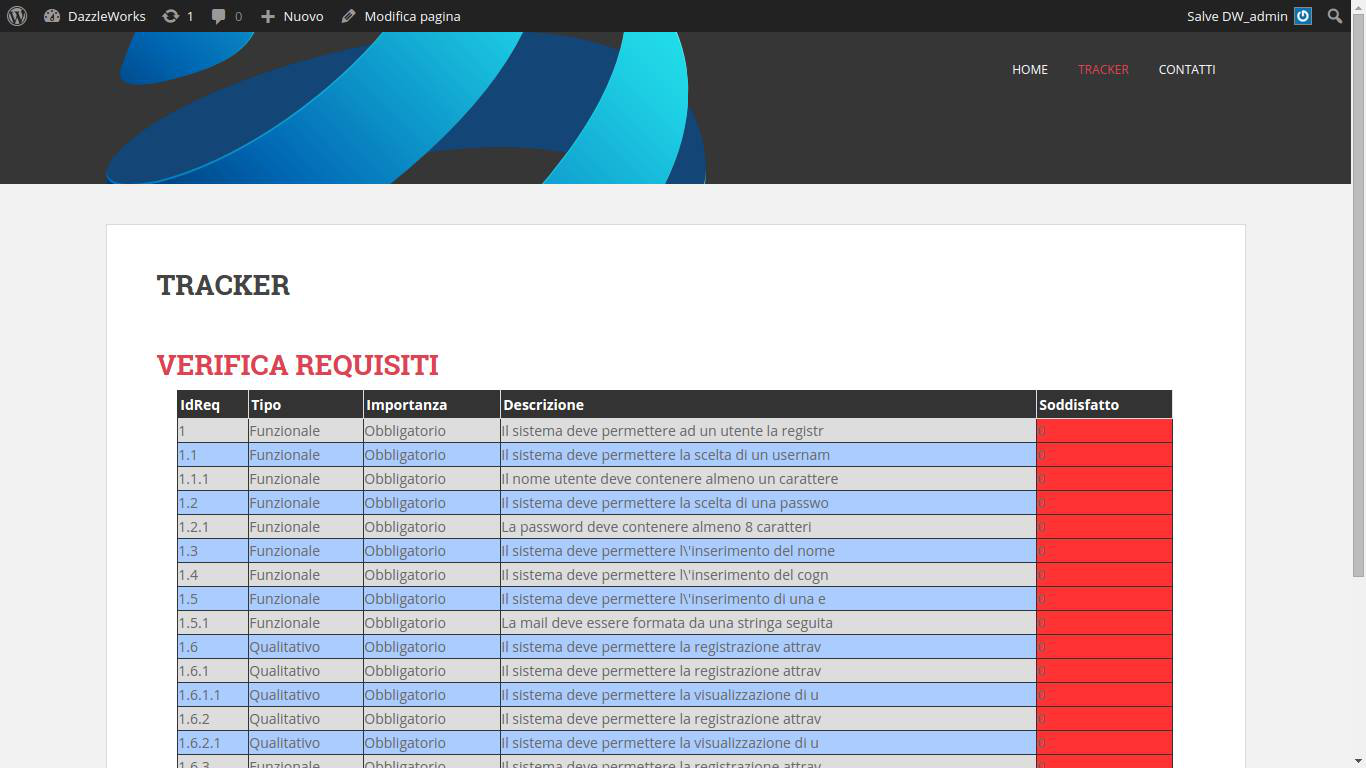
\includegraphics[width=0.7\linewidth]{img/tracker1}
\caption[Pagina riepilogo requisiti]{Pagina riepilogo requisiti}
\label{fig:tracker1}
\end{figure}
\begin{figure}[h]
\centering
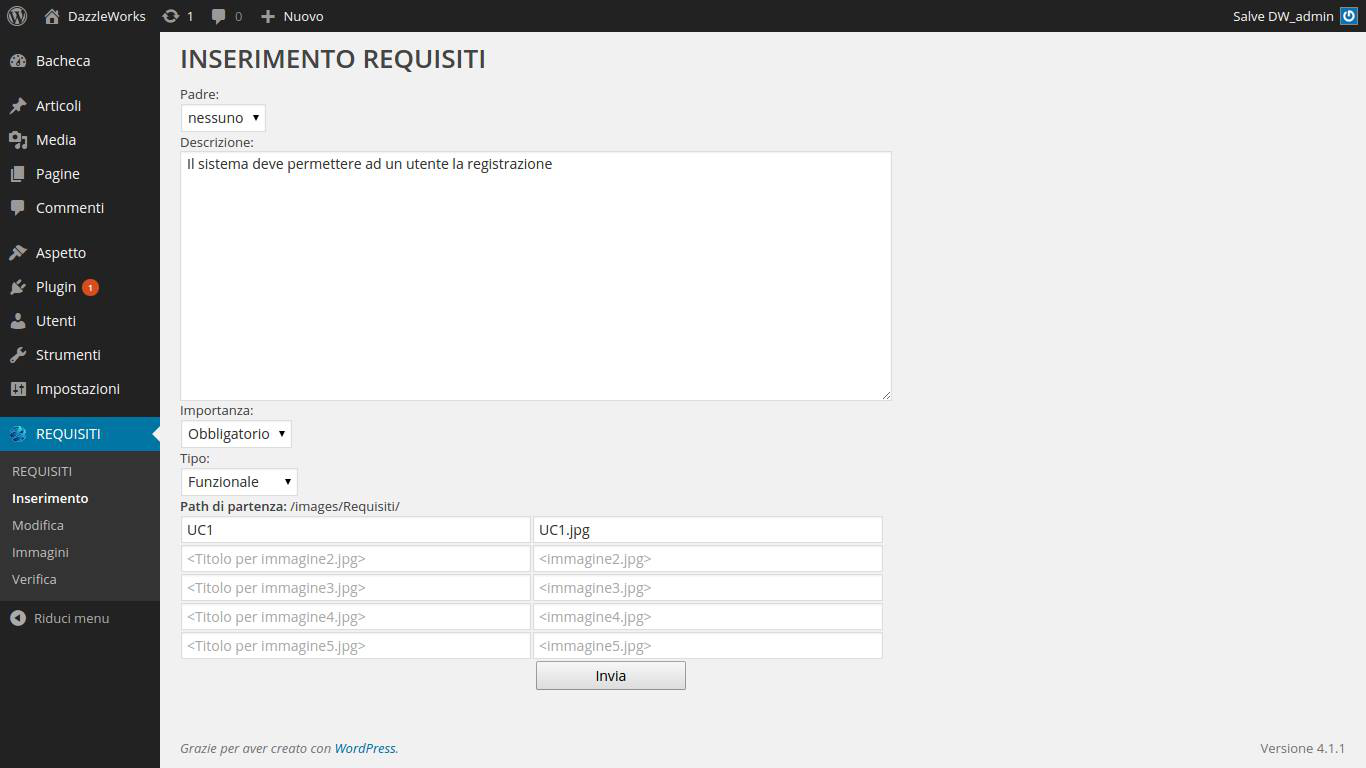
\includegraphics[width=0.7\linewidth]{img/tracker2}
\caption[Pagina inserimento requisito]{Pagina inserimento requisito}
\label{fig:tracker2}
\end{figure}




\newpage
\section{Progettazione}
Dopo la fase di \textbf{Analisi} si passerà alla fase di \textbf{Progettazione} dove i \textit{Progettisti} dovranno seguire le seguenti regole.\\
\paragraph{Diagrammi UML}
Dovranno essere realizzati i seguenti diagrammi:
\begin{itemize}
	\item Diagrammi delle classi;
	\item Diagrammi dei package;
	\item Diagrammi delle attività;
	\item Diagrammi di sequenza.
\end{itemize}
La lingua utilizzata nella realizzazione dei diagrammi sarà l'\textbf{inglese} e lo standard \gls{UML} sarà 2.0.

\paragraph{Design Pattern}
I \textit{Progettisti} dovranno utilizzare il \gls{design pattern} che ritengono più adatto al contesto per rendere l'applicazione più efficiente possibile. Ogni \gls{design pattern} utilizzato verrà accompagnato da una breve descrizione e da un diagramma che ne esemplifica il funzionamento.

\paragraph{Classi di verifica}
Andranno create delle classi di verifica per testare che tutti i componenti abbiano un comportamento corretto.

\paragraph{Stile di progettazione}
Durante la fase di \textbf{Progettazione} bisognerà fare attenzione a:
\begin{itemize}
	\item \textbf{Ricorsione}: non dovrà essere utilizzata la ricorsione a meno che non sia strettamente necessaria. In quel caso dovrà essere fornita una dimostrazione induttiva sulla correttezza del metodo in questione;
	\item \textbf{Annidamento di cicli}: all'interno di un metodo non dovranno esserci cicli annidati con una profondità maggiore a cinque.
\end{itemize}






%\newpage
%\section{Codifica e Convenzioni}
%\subsubsection{Linguaggi di codifica}
Dopo un'analisi del capitolato d'appalto e dei requisiti si è deciso che per lo sviluppo del software richiesto si utilizzeranno i linguaggi \gls{HTML5} , \gls{PHP} e \gls{Javascript}.

\subsubsection{Framework e librerie}
Per semplificare la realizzazione della nostra applicazione web si è deciso di utilizzare il \gls{framework} \gls{Angular}, per migliorare le interfacce utente, e la libreria \gls{Chart.js}, utilizzata per generare grafici.

\subsubsection{Convenzioni di codifica}
Di seguito è riportato l'insieme di norme e convenzioni che il gruppo dovrà seguire nella scrittura e documentazione del codice.
L'unica lingua ammessa per i nomi di variabili, metodi e commenti è l'inglese.

\subsubsection{File HTML}

Ogni file \gls{HTML} deve iniziare con il tag <!DOCTYPE html> che serve ad indicare che verrà utilizzata la versione \gls{HTML5}.
Ogni tag deve contenere un id e può contenere una o più classi.
Gli id e le classi dovranno essere contenute in un file .css a parte per mantenere il più possibile la separazione tra \gls{layout} e contenuto.
Le pagine \gls{HTML} devono rispettare gli standard del \gls{W3C}.

\subsubsection{Nomenclatura}
Per l'assegnazione di nomi a variabili, metodi e costanti andranno seguite le seguenti regole:
\begin{itemize}
	\item \textbf{Funzioni:} va utilizzata la notazione mixed case, con la prima lettera minuscola;
	\item \textbf{Variabili:} va utilizzata la notazione mixed case, con la prima lettera minuscola;
	\item \textbf{Costanti:} va scritto il nome interamente in maiuscolo, separando le varie parole con il carattere "\_" (underscore).
\end{itemize}

\subsubsection{Intestazione di un file Javascript}

\begin{flushleft}

/*\\
\vspace{3mm}
\begin{tabular}{l}
	File\\
	Autore\\
	Data\\
	Descrizione\\
\end{tabular}\\
\vspace{5mm}
 Modifiche:\\
 \vspace{3mm}
\begin{tabular}{| c c c c c c c c c |}
	\hline
	Versione & - & Data & - & Programmatore & - & Modifica & - & Descrizione\\
	\hline
	x.y.z & - & aaaa-mm-gg & - & Nome Cognome & - & Funzione & - & Descrizione modifica\\
	\hline
\end{tabular}\\
\vspace{3mm}
*/\\

\end{flushleft}

\begin{itemize}
	\item \textbf{File:} nome del file;
	\item \textbf{Autore:} nome e cognome del creatore del file;
	\item \textbf{Data:} data di creazione del file nel formato aaaa-mm-gg;
	\item \textbf{Descrizione:} poche righe di descrizione delle funzionalità contenute nel file;
	\item \textbf{Cambiamenti:} tabella dello stato di avanzamento del file, contenente tutte le modifiche effettuate :
		\begin{itemize}
			\item \textbf{Versione:} versione una volta effettuata la modifica;
			\item \textbf{Data:} data della modifica;
			\item \textbf{Programmatore:} nome e cognome del programmatore che ha effettuato la modifica;
			\item \textbf{Modifica:} segnatura della funzione a cui è stata apportata una modifica;
			\item \textbf{Descrizione:} breve descrizione della modifica effettuata.
		\end{itemize}
\end{itemize}

\subsubsection{Commenti}

Prima di ogni funzione dovrà essere presente un commento con la seguente forma:

\begin{flushleft}
/*\\
\vspace{3mm}
\begin{tabular}{l}
	Descrizione della funzione\\
	Descrizione dei parametri\\		
	Descrizione del tipo di ritorno\\
\end{tabular}\\
\vspace{3mm}
*/

\end{flushleft}

Ogni variabile di particolare importanza dovrà essere fornita di commento che ne spieghi scopo e funzionamento.



\newpage
\appendix
\section{Lista di controllo}
Di seguito verrà presentata la lista degli errori più comuni trovati durante le verifiche dei documenti:
\begin{itemize}
	\item \textbf{Norme stilistiche:} la conoscenza \textbf{non} approfondita delle norme per la stesura dei documenti potrebbe portare a errori:
		\begin{itemize}
			\item Nel caso degli elenchi potrebbero esserci elementi che non iniziano con la lettera maiuscola;
			\item Nel caso degli elenchi potrebbe non terminare con il "." nel caso dell'ultimo elemento oppure potrebbe mancare il ";" per uno o più elementi tranne l'ultimo; 
			\item Potrebbe mancare la marcatura "G" in pedice per i termini presenti nel \textit{Glossario};
			\item Il non utilizzo del grassetto per le fasi principali del progetto, il corsivo per i documenti e i ruoli di progetto;
			\item Le note a piè di pagina che non iniziano con una maiuscola e non finiscono con il ".".
		\end{itemize}
	\item \textbf{Lingua italiana:} 
		\begin{itemize}
			\item Più tempi verbali all'interno della stessa frase;
			\item Utilizzo di termini con significato ambiguo.
		\end{itemize}
	\item \textbf{\LaTeX:} non viene considerato il carattere di spaziatura dopo l'inserimento dei  comandi \LaTeX;
	\item \textbf{Altro:} errori dovuti a distrazioni e/o errori di battitura.
\end{itemize}



%\newpage

% ...

%\printglossaries

\end{document}
